\documentclass{article}
\usepackage[utf8]{inputenc}
\usepackage{geometry}
 \geometry{
 a4paper,
 total={170mm,257mm},
 left=20mm,
 top=20mm,
 }


\title{Operator Product Expansion}
\author{Luigi Del Debbio, Joseph Lee, Andrew Yong}
\date{January 2019}

\usepackage{natbib}
\usepackage{graphicx}
\usepackage{amsmath}
\usepackage{amssymb}
\usepackage{textcomp}
\usepackage{empheq}
\usepackage{physics}
\usepackage{tikz-feynman}
\setcitestyle{square}

\begin{document}

\maketitle
\renewcommand{\abstractname}{\vspace{-\baselineskip}}
\begin{abstract}
These notes aim to supplement Collin's discussion on Operator Product Expansion (Ch.10, Renormalisation\cite{collins_1984}). Useful reference \cite{schwartz}
\end{abstract}

\section{Divergent Example - \S 10.1.2}
In \S10.1, we have been exploring the expansion of the two point function $T\phi(x)\phi(0)$. As explained at the end of \S10.1.1, we will be restricting our attention to the leading-power behaviour, i.e. studying
\begin{align*}
    T\phi(x)\phi(0) \sim C_{\phi^2}(x)[\phi^2]
\end{align*}
where $[\phi^2]$ is the renormalized Green's function. \\

In this `divergent example', we evaluate the correction to $T\phi(x)\phi(0)$. At order $\mathcal{O}(g)$, the correction is given by
\begin{equation}
    \frac{i^2}{(p_1^2-m^2)(p_2^2-m^2)}ig\int \frac{d^4q}{(2\pi)^4} \frac{e^{-iq\cdot x}}{(q^2-m^2)((q-p_1-p_2)^2 - m^2)}.
    \label{loopOg}
\end{equation}
which corresponding feynman diagram is 10.1.3(a).\\

Two regions of momentum $q$ contribute differently to this term:
\begin{enumerate}
    \item $q$ finite as $x \rightarrow 0$, this  provides an $x-$independent correction,
    \item $q$ large (up to $O(1/x)$) as $x \rightarrow 0$, this  provides an $x-$dependent correction.
\end{enumerate}
As we will see, this allows us to express 
\begin{align}
    C_{\phi^2} = 1 + (g/16\pi^2)c_1(x^2)
\end{align}
where the two regions contribute to the two terms respectively. The two terms correspond to the decomposition of fig  10.1.13(a) into (b) and (c), where (b) is simply performing renormalization to $\phi(0)^2$ by cutting off the UV divergence, and (c) takes care of the remaining contribution. 
\subsection{Momentum region 1: $q$ finite, $x\rightarrow 0$}

In the region where $q$ is finite, sending $x\rightarrow 0$ (so $e^{-iq\cdot x} \rightarrow 1$) will get  us the standard logarithmic divergent term of the form 

\begin{equation}
    \frac{i^2}{(p_1^2-m^2)(p_2^2-m^2)}ig\int \frac{d^4q}{(2\pi)^4} \frac{1}{(q^2-m^2)((q-p_1-p_2)^2 - m^2)}.
    \label{logdiv}
\end{equation}

To renormalise this, we can use dimensional regularisation to expose the divergent terms. First, we apply the Feynman parameter trick to Equation \ref{logdiv},

\begin{equation}
    \frac{1}{AB} = \int_0^1 dx \, \frac{1}{(A(1-x) + Bx)^2}.
\label{Feynparam trick}
\end{equation}
Identifying $A=(q^2-m^2)$ and $B=((q-p)^2-m^2)$, with $p=p_1+p_2$, the integral in Equation \ref{logdiv} becomes

\begin{equation}
\begin{split}
    I(p) &= ig\int \frac{d^4q}{(2\pi)^4}\int^1_0 dx \frac{1}{((q^2-m^2)(1-x) +(q-p_1-p_2)^2 - m^2)x)^2},\\
    &= ig\int \frac{d^4q}{(2\pi)^4}\int^1_0 dx \frac{1}{((q-px)^2 + p^2x(1-x) - m^2 )^2},\\
    \mathrm{let}\, q'&= q-px,\\
    &= ig\int \frac{d^4q}{(2\pi)^4}\int^1_0 dx \frac{1}{(q^2 -M^2)},
    \label{b4dimreg}
\end{split}
\end{equation}
where $M^2=M^2(s,m)=m^2-sx(1-x)$ and $s$ is the centre-of-mass energy, $s=p^2$.

Next, we can Wick rotate to Euclidean momenta and generalise this integral to $D$-dimensions. This is captured by the following identity, 
\begin{equation}
    \int\frac{d^Dq}{(2\pi)^D} \frac{q^{2a}}{(q^2-M^2)^b}=\frac{i}{(4\pi)^{D/2}}\frac{(-1)^{a-b}}{(M^2)^{b-a-D/2}} \frac{\Gamma(a+\frac{D}{2})\Gamma(b-a-\frac{D}{2})}{\Gamma(b)\Gamma(\frac{D}{2})}
\end{equation}
which is proven in the Appendix\footnote{if it exists.}. Here, $\Gamma(x)$ is the gamma function, where $\Gamma(x) = (x-1)! = (x-1)\Gamma(x-1)$, with $\Gamma(1)=1$. Moreover, for $D\neq 4$, the coupling $g$ for a $\phi^4$ theory will be dimensionful. We can keep $g$ dimensionless by performing the replacement
\begin{equation}
    g \rightarrow \mu^{4-D}g.
\end{equation}
Identifying $a=0$ and $b=2$ in Equation \ref{b4dimreg}, we have 

\begin{equation}
    \begin{split}
        I(p) &= ig\mu^{4-D} \frac{i}{(4\pi)^{D/2}}\frac{\Gamma(\frac{D}{2})\Gamma(2-\frac{D}{2})}{\Gamma(2)\Gamma(\frac{D}{2})}\int^1_0 dx \, \frac{(-1)^{-2}}{(M^2)^{2-D/2}},\\
        &= ig\mu^{4-D} \frac{i}{(4\pi)^{D/2}}\Gamma(2-\frac{D}{2})\int^1_0 dx \, \frac{1}{(M^2)^{2-D/2}},\\
    \end{split}
\end{equation}

Now, we let $D=4-2\epsilon$. Then, $I(p)$ becomes

\begin{equation}
    I(p)=ig\frac{i}{16\pi^2}(4\pi)^{\epsilon}\Gamma(\epsilon)\int^1_0 dx \, \left(\frac{\mu^2}{M^2}\right)^{\epsilon},
\end{equation}

Recall that, in the limit of $\epsilon\rightarrow 0$, we can make the following approximation:

\begin{equation}
\begin{split}
    u^\epsilon &= 1 + \epsilon \log{u} + \mathcal{O}(\epsilon),\\
    \Gamma(\epsilon) &= \frac{1}{\epsilon} - \gamma_E + \mathcal{O}(\epsilon),
\end{split}
\end{equation}
where $u$ is some polynomial of order $\epsilon$ and $\gamma_E$ is the Euler-Mascheroni constant.

Using the relations above, $I(p)$ becomes

\begin{equation}
    \begin{split}
       I(p)&=ig\frac{i}{16\pi^2}\int^1_0 dx \, (1+\epsilon\log{4\pi} + \mathcal{O}(\epsilon))(\frac{1}{\epsilon} - \gamma_E + \mathcal{O}(\epsilon))(1+\epsilon\log{\frac{\mu^2}{M^2}}+ \mathcal{O}(\epsilon)),\\
       &=ig\frac{i}{16\pi^2}\int^1_0 dx \, \frac{1}{\epsilon} - \gamma_E + \log{\frac{4\pi\mu^2}{M^2}} + \mathcal{O}(\epsilon).
    \end{split}
\end{equation}

Now, we apply the MS subtraction scheme, where the $\epsilon$ terms are removed from the integral. At last, Equation \ref{loopOg} becomes 

\begin{equation}
     \frac{i^2}{(p_1^2-m^2)(p_2^2-m^2)}\frac{-g}{16\pi^2}\int^1_0 dx \, \log{\frac{4\pi\mu^2}{M^2}} - \gamma_E.
\end{equation}
And this is the order 1 contribution to the correction from the first momentum region.

\subsection{Momentum region 2: large $q \sim O(1/x)$}\label{large q}
The remaining contribution is in equation (10.1.13):
\begin{equation} \label{eq:div_eg_large_q}
    \frac{i^2}{(p_1^2-m^2)(p_2^2-m^2)}\frac{ig}{(2\pi)^4}\cross\qty{\int d^4q \frac{e^{iq\cdot x}-1}{(q^2-m^2)[(q-p_1-p^2)^2-m^2]}-\text{UV divergence}}
\end{equation}
For this term, the second region of momentum, where $q$ becomes large up to $O(1/x)$ as $x \rightarrow 0$, is important, since it provides a contribution of order 1 (as $q\cdot x \sim 1$), whereas the first region (finite $q$) only has a contribution of order $\abs{x}$. We again note that, as will be shown, the UV divergence here is equal to that present in the first region, and therefore the decomposition makes sense. 

As we are considering large $q \sim 1/x$, we can see that $p_1$, $p_2$ and $m$ does not provide leading-power contribution to the term in the curly-bracket (differentiating the term w.r.t $p_1$, $p_2$ or $m$ will always bring another power of $q$ to the denominator, which results in a convergent finite integral, which goes to $0$ as some power of $x$ when $x \rightarrow 0$). We can therefore ignore these variables and set $m=p_1=p_2=0$ in defining $c_1$. \\

Consider the term
\begin{equation}
\begin{split}
    &\ \text{i}\int d^4q\frac{e^{iq\cdot x}-1}{(q^2)^2} \\
    &\rightarrow\frac{\text{i}}{(2\pi\mu)^{D-4}}\int d^Dq\frac{e^{iq\cdot x}-1}{(q^2)^2} \text{ - analytically continue to dim D, with } g \rightarrow \mu^{4-D}g\\
    &= \frac{\text{ig}}{(2\pi\mu)^{D-4}}\int d^Dq \int_0^\infty  dz\ z e^{-z(-q^2)} e^{iq\cdot x}-1) \text{ - using identity provided}\\
    &= \frac{-1g}{(2\pi\mu)^{D-4}}\int d^Dq \int_0^\infty  dz\ z e^{-z(q^2)} (e^{-iq\cdot x}-1) \text{ - wick rotation}\\
    &= \frac{-1}{(2\pi\mu)^{D-4}}\int d^Dq \int_0^\infty  dz\ z (e^{-z(q^2+iq\cdot x/z+(ix/2z)^2)-x^2/4z}-e^{-z(q^2)}) \text{ - complete the square}\\
    &= \frac{-1}{(2\pi\mu)^{D-4}}\int d^Dq \int_0^\infty  dz\ z (e^{-z(q+ix/2z)^2}e^{-x^2/4z}-e^{-z(q^2)})\\
    &= \frac{-1}{(2\pi\mu)^{D-4}}\int_0^\infty  dz\ z (\frac{\pi}{z})^{D/2}(e^{-x^2/4z}-1)\text{ - gaussian integral}\\
\end{split}
\end{equation}

substitute $t = \frac{x^2}{4z},\ dz=-\frac{x^2}{4t^2}dt,\ \int_0^\infty \rightarrow \int_\infty^0$
\begin{equation}
\begin{split}    
    &= \frac{-1}{(2\pi\mu)^{D-4}}\int_0^\infty  dt\ \frac{x^2}{4t^2} \frac{x^2}{4t}
    (\frac{4\pi t}{x^2})^{D/2}(e^{-t}-1)\\
    &= \frac{-\pi^{D/2}(x^2)^{2-D/2}}{(2\pi\mu)^{D-4}4^{2-D/2}}\int_0^\infty  dt\ t^{D/2-3}(e^{-t}-1)
\end{split}
\end{equation}
using $\Gamma(z)=\int_0^\infty dt\ t^{z-1}e^{-t}$
\begin{equation}
    = \frac{-\pi^{D/2}(x^2)^{2-D/2}}{(2\pi\mu)^{D-4}4^{2-D/2}}(\Gamma(\frac{D}{2}-2)-\eval{\frac{t^{D/2-2}}{D/2-2}}_0^\infty )
\end{equation}
using the property that $\int d^Dp(p^2)^\alpha = 0$ (see Collins, p.73 eq 4.3.1a), we see that the second term vanishes. Now, we set $D=4-2\epsilon$
\begin{equation}
\begin{split}
    &= \frac{-\pi^{2-\epsilon}(x^2)^{\epsilon}}{(2\pi\mu)^{-2\epsilon}2^{2\epsilon}}\Gamma(-\epsilon)\\
    &= -\pi^2(\pi\mu^2 x^2)^\epsilon\Gamma(-\epsilon)\\
    &= -\pi^2 (1+\epsilon \ln(\pi \mu^2 x^2)+O(\epsilon^2))(-\frac{1}{\epsilon}-\gamma+O(\epsilon))\\
    &= \pi^2(\frac{1}{\epsilon}+\gamma+\ln(\pi\mu^2 x^2)+O(\epsilon))\\
    &= \pi^2(\frac{1}{\epsilon}+\gamma+\ln(-\pi\mu^2 x^2)+O(\epsilon))\text{ - Wick rotate back}
\end{split}
\end{equation}

Therefore
\begin{equation}
    \frac{ig}{(2\pi)^4}\cross\qty{\int d^4q \frac{e^{iq\cdot x}-1}{(q^2-m^2)[(q-p_1-p^2)^2-m^2]}} = \frac{1}{16\pi^2}\qty{\frac{1}{\epsilon}+\gamma+\ln(-\pi\mu^2 x^2)}
\end{equation}
As we can see, this term has the same pole/UV-divergence as that from the first region, and so the decomposition makes sense. And now we can identify
\begin{equation}
\begin{split}
    c_1(x) &= \frac{1}{2\pi^2} \qty{\frac{\text{i}}{(2\pi\mu)^{D-4}}\int d^Dq\frac{e^{iq\cdot x}-1}{(q^2)^2}-\frac{2}{D-4}}\\
    &=\frac{1}{2\pi^2} \qty{\pi^2(\frac{1}{\epsilon}+\gamma+\ln(\pi\mu^2 x^2)+O(\epsilon))-\frac{1}{\epsilon}}\\
    &=\frac{1}{2}(\gamma+\ln(-\pi\mu^2 x^2))
\end{split}
\end{equation}

\section{Strategy of proof}
\subsection{Weinberg's theorem}
In the diveregnt example, we have seen how to treat the contribution from the large $q$ region for the specific diagram. There we can easily see that the leading order $q$ contribution (equation \ref{eq:div_eg_large_q}) has to come from the single loop, then can we argue from there that the leading power contibution from the loop does not depend on the external momenta/mass. In this case, identifying and isolating the large $q$ behaviour is easy. To be able to generalise the discussion to any diagrams, we have to understand the behaviour of a general graph when the internal momentum $q$ is large; this is where Weinberg's theorem \cite{weinberg} comes in. In essence, Weinberg's theorem allows us to identify and isolate/factorise the largest power contribution from a given diagram. Before we can discuss the theorem itself, we have to understand the concept of subgraph.\\



\subsubsection{Subgraphs}
Definition: A set $\mathcal{G'}$ of internal and external lines $j$ form a subgraph of $\mathcal{G}$ provided that there is no vertex in $\mathcal{G}$ to which is attached just one line of those in $\mathcal{G'}$. In other words, a subgraph $\mathcal{G'}$ is composed of a number of paths which begin and end in external lines or each other, but never end abruptly within $\mathcal{G}$. 

\subsubsection{Example of subgraphs}
For this diagram:\\
\feynmandiagram [small, horizontal=a to b] {
i1 -- [plain] a -- [plain] c -- [plain] i3,
i2 -- [plain] b -- [plain] d -- [plain] i4,
a -- [photon] b,
d -- [photon] c,
};\\
Subgraphs include:\\
\feynmandiagram [small, horizontal=a to b] {
i1 -- [plain, very thick] a -- [plain, very thick] c -- [plain, very thick] i3,
i2 -- [plain] b -- [plain] d -- [plain] i4,
a -- [photon] b,
d -- [photon] c,
};
\feynmandiagram [small, horizontal=a to b] {
i1 -- [plain, very thick] a -- [plain] c -- [plain, very thick] i3,
i2 -- [plain] b -- [plain, very thick] d -- [plain] i4,
a -- [photon, very thick] b,
d -- [photon, very thick] c,
};
\feynmandiagram [small, horizontal=a to b] {
i1 -- [plain, very thick] a -- [very thick, plain] c -- [plain, very thick] i3,
i2 -- [plain] b -- [plain, very thick] d -- [plain] i4,
a -- [photon, very thick] b,
d -- [photon, very thick] c,
};...\\

\subsubsection{Theorem}
Consider a Feynman diagram $\mathcal{G}$ in any local field theory. Any external or internal lines $j$ in this diagram is associated with a bare propagator $\Delta_j(p_,j\sigma)$, where $p_j$ is the four-momentum carried by the line $j$, and $\sigma$ is the label that contains all discrete variables such as spins, polarizations, etc. The integrand $F$ corresponding to the diagram $\mathcal{G}$  is given as the product
\begin{equation}
    F= \gamma(\sigma)\prod_{j=1}^M \Delta_j(p_,\sigma)
\end{equation}
over all lines $M$. $\gamma(\sigma)$ here is the product of all vertex factors including Dirac matrices, coupling constants etc. \\

The Green's function corresponding to $\mathcal{G}$ is given by the integrating $F$ over the internal momenta:

\begin{equation}
    G(\mathbf{P}\in E, \sigma_{ext}) = \sum_{\sigma_{int}}\int_{\mathbf{P'}\in I}F(\mathbf{P+P'},\sigma) d\mathbf{P'}
\end{equation}
Here $E(I)$ denotes the subspace of external (internal) momenta.\\

The theorem tells us that for the integral $G$ (with Wick rotated contour):
\begin{enumerate}
    \item $G$ converges if 
    \begin{enumerate}
        \item it converges superficially (i.e. $D_I:=\alpha(I)+\text{dim}I<0$) and 
        \item all sub-integrations converge superficially (i.e. $D_{I'}=\alpha(I')+\text{dim}I'<0$ for $I'\subset I$)
    \end{enumerate}
\end{enumerate}
Here $D_I$ is the superficial degree of divergence of the integral, and the asymptotic coefficient $\alpha(S)$ is defined by $F(\mathbf{L}\eta+\mathbf{C}) = O(\eta^{\alpha(\mathbf{L})})$ for $\mathbf{L}\in S$, i.e. the power scaling with a momentum vector in $V$. (for complete definition, see \cite[\S III]{weinberg})

\begin{enumerate}
\setcounter{enumi}{1}
    \item For any $S \subset E$, the asymptotic coefficient of $G$: $\alpha_I(S)=\max\limits_{\mathcal{G'}\ni S} \mathcal{D}_I(\mathcal{G'})$, where the max here is over all subgraphs $\mathcal{G'}$ which contains just the set $\mathcal{E}_\infty$ of external lines $j$ for which $\mathbf{V}_j$ is not orthogonal to $S$ (this condition is true for `almost any' choice of $p_j$, detail see \cite[\S V]{weinberg}). 
\end{enumerate}
Here $\mathcal{D}_I$ is called the dimensionality, and it is the net number of momentum factors of the subgraph $\mathcal{G'}$, counting the momentum power $\alpha_j$ for each line $j$ ($-2$ for boson and $-1$ for fermion) and 4 for each integration. 

In other words, the second part of the theorem tells us that for a graph $\mathcal{G}$, if we let the momentum of a set of external lines $\mathcal{E}_\infty$ go to infinity, then the integrated Green's function corresponding to $\mathcal{G}$ will behave as $O\{\eta^{\alpha_I(\mathcal{E}_\infty)}(\log \eta)^{\beta_I(\mathcal{E}_\infty)}\}$, where $\alpha_I(\mathcal{E}_\infty)$ is the maximum of the dimensionality of all subgraphs $\mathcal{G'}$ of $\mathcal{G}$ including the external lines $\mathcal{E}_\infty$ and no other external lines.

\subsubsection{Example}
Let us try to figure out the behaviour of this graph as $k \rightarrow \infty$:\\
\feynmandiagram [small, horizontal=a to b] {
i1 -- [fermion, edge label=\(k\)] a -- [fermion, edge label=\(k+p-q\)] c -- [fermion, edge label=\(k+p-p'\)] i3,
i2 -- [fermion, edge label'=\(p\)] b -- [fermion, edge label'=\(q\)] d -- [fermion, edge label'=\(p'\)] i4,
a -- [photon, edge label'=\(q-p\)] b,
d -- [photon, edge label'=\(q-p'\)] c,
};\\
The corresponding integral (excluding external legs) is roughly (ignoring vertex and gamma factors/slashes etc.):
\begin{equation}
\begin{split}    
    \int \frac{d^4q}{(2\pi)^4}\frac{k+p-q}{(k+p-q)^2+m^2}\frac{k+p-p'}{(k+p-p')^2+m^2}\frac{1}{(q-p')^2+\mu^2}\frac{1}{(q-p)^2+\mu^2}\frac{q}{q^2+m^2}
\end{split}
\end{equation}
Part 2 of the theorem tells us to look at all subgraphs with the two external legs containing $k$, i.e. the two external legs on the left hand side, and no other external legs. This gives us the three subgraphs we presented before:\\
a:
\feynmandiagram [small, horizontal=a to b] {
i1 -- [fermion, very thick] a -- [fermion, very thick] c -- [fermion, very thick] i3,
i2 -- [fermion] b -- [fermion] d -- [fermion] i4,
a -- [photon] b,
d -- [photon] c,
};
b:
\feynmandiagram [small, horizontal=a to b] {
i1 -- [fermion, very thick] a -- [fermion] c -- [fermion, very thick] i3,
i2 -- [plfermionain] b -- [fermion, very thick] d -- [fermion] i4,
a -- [photon, very thick] b,
d -- [photon, very thick] c,
};
c:
\feynmandiagram [small, horizontal=a to b] {
i1 -- [fermion, very thick] a -- [very thick, fermion] c -- [fermion, very thick] i3,
i2 -- [fermion] b -- [fermion, very thick] d -- [fermion] i4,
a -- [photon, very thick] b,
d -- [photon, very thick] c,
};\\
The dimensionality of each graph could be calculated by summing $-2$ for each internal boson line, $-1$ for each internal fermion line and $4$ for each loop:
\begin{equation}
\begin{split}
    &\mathcal{D}_a= -1,\\ &\mathcal{D}_b= -2-1-2=-5,\\ &\mathcal{D}_c= -1-1-2-2+4=-2,  
\end{split}
\end{equation}
The maximum is $\mathcal{D}_a= -1$, therefore as $k \rightarrow \infty$, the integral goes as $k^{-1}$ (times some log). 

\subsection{Strategy of proof}
\subsubsection{Large $q$ subgraphs: $U$}
Weinberg's theorem tells us that to identify the leading power behaviour of a diagram when the momentum $q$ is large, we have to look at the subgraph with the largest power of momentum. In the case of our OPE expansion (in momentum space), we have to consider those subgraphs which contains $\phi(q)$ and $\phi(0)$ as external legs. 

For our scalar $\phi^4$ theory, we can show that subgraphs with the greatest power of momentum must only have 2 extra external legs other than $\phi(0)$ and $\phi(q)$. We can see this by using the usual divergence counting method:
\begin{equation}
\begin{split}
    &D=4L-2P\\
    &L=P-V\\
    &V=\frac{1}{4}(2P+E)\\
    &\rightarrow D=-E
\end{split}
\end{equation}
where $D$ is the degree of divergence, $L$ the number of loops, $P$ the number of propagators, $E$ number of external legs and $V$ number of vertices. We therefore want the subdiagram with as few external lines as possible; in our case, it will be 4, i.e. 2 extra external legs. 

Because of this, the subgraphs contributing to the leading power $q$ will take the form of the subgraph U in Fig. 10.2.1, in which all lines carry momentum of order $q$, with two lines connecting to the IR subgraph I. 

Since the UV subgraph U is, to the leading power of $q^2$, independent of the external momenta $k$ and $l$ flowing into it, we may replace U by its value when $k=l=m=0$, and replace the IR subgraph I by an insertion of a vertex for $\phi^2/2$ in the Green's function. This allows us to factorise the two leg UV subgraph from the rest of the N-point IR diagram. At large $q$, we only need to care about U with the 2 extra external lines. This is why the diagram in Fig 10.1.3 (a) is representative and highly relevant to the OPE, as it is itself of the form U.

\subsubsection{Constructing Wilson Coefficients}
Now to actually construct the expansion, we have to consider the leading contribution when all the momenta in U is large. In the case where we have large momenta contained within a proper subregion of U, the contribution of U to the Wilson coefficient is defined such that these contributions are subtracted out, as in equation 10.2.2. We are then ready to use the technique applied to Fig. 10.1.3 on U, where we evaluated and integrate Fig 10.1.3 (c) at $k=l=m=0$ to obtain the leading order contribution to the Wilson coefficient at large $q$. 

\section{Proof}

Now, we will prove the operator product expansion using $\phi^4$-theory as a concrete example. As a reminder, consider the Green's function

\begin{equation}
    G_{N+2}(x, p_1,\dots, p_n) = \mel{0}{T\phi(x)\phi(0)\Tilde{\phi}(p_1)\dots\Tilde{\phi}}{0},
\end{equation}
where each $\phi(x)$ and $\phi(0)$ is connected to some external line. If we rescale $x \rightarrow kx$, for some scale, $k$, we can construct a general decomposition of the form:

\begin{equation}
    G_{N+2}(kx, p_1,\dots, p_n) = C(k^2x^2)\mel{0}{T\frac{1}{2}\phi(0)^2\Tilde{\phi}(p_1)\dots\Tilde{\phi}}{0} + r_{N+2}(kx,p_1,\dots,p_N),
    \label{green's decomposed}
\end{equation}
for some remainder term, $r_{N+2}$.     

We note that, in every order of perturbation theory, the coefficient $C(k^2x^2)$ behaves like $(k^2)^0\log f(k)$ when the scaling parameter $k\rightarrow 0$, while the remainder $r_{N+2}\rightarrow0$ like the power of $k$. On the other hand, if we examine the Green's function in momentum space, we have 

\begin{equation}
    G_{N+2}(kx, p_1,\dots, p_n) = \Tilde{C}(q^2/k^2)\mel{0}{T\frac{1}{2}\phi(0)^2\Tilde{\phi}(p_1)\dots\Tilde{\phi}}{0} + r_{N+2}(q/k,p_1,\dots,p_N).
    \label{green with remainder}
\end{equation}
Now, recall the definition of the Fourier transform

\begin{equation}
    G_{N+2}(kx,p_1,\dots,p_N) = \int \frac{d^4q}{(2\pi)^4} \, e^{-iq\cdot x} \, \Tilde{G}_{N+2}(q/k,p_1,\dots,p_N).
    \label{green with remainder in momentum}
\end{equation}
We find that $\mathrm{dim}\,\Tilde{G} = \mathrm{dim}\,G-4$ and therefore $\mathrm{dim}\,\Tilde{C}(q/k) = \mathrm{dim}\,C(kx)-4$. Since the coefficients in position space are dimensionless, we find that $\mathrm{dim}\,\Tilde{C}(q/k)=4$. Thus, when we send the scaling parameter $k\rightarrow 0$, or $q/k \rightarrow \infty$, we will find that $\Tilde{C}(q/k)$ behaves like $(q/k)^4 \log f(k) $ and the remainder term vanishes by a smaller power of $k$. 

\subsection{Construction of the Remainder}

As mentioned before, we will work in $\phi^4$-theory as an example, but this can be generalised with  some effort. In any case, the Lagrangian is the usual

\begin{equation}
    \mathcal{L}= \frac{1}{2}\partial_\mu\phi\partial^\mu\phi - \frac{1}{2}m^2\phi^2 - \frac{g}{4!}\phi^4.
\end{equation}

Let $\Gamma$ represent the Feynman graph we are interested in. The renormalised graph, which we will call $R(\Gamma)$, is $\Gamma$ minus the counterterms which subtract away the UV divergences. Then, $R(\Gamma)$ is a contribution of $\Gamma$ to the Green's function, $G_{N+2}$. Looking back at Equation \ref{green's decomposed}, we still have the remainder term to consider. Let's call it $r(\Gamma)$. This remainder term contains other counterterms that remove not only the UV divergent terms but also the leading $x\rightarrow 0$ or $q \rightarrow \infty$ behaviour of $\Gamma$. In this sense, $R(\Gamma) - r(\Gamma)$ will give us the Wilson coefficient, that is, the first term in Equation \ref{green with remainder} and \ref{green with remainder in momentum}.

To determine what form does $r(\Gamma)$ take, we must first understand how the renormalised graph, $R(\Gamma)$, is constructed. Recall that UV divergences arise from regions with high loop momenta. We employ the following expression to represent the standard programme of regularisation,

\begin{equation}
    R(\Gamma) = \Gamma - \sum_\gamma C_\gamma(\Gamma),
\end{equation}
where the sum is over all subgraphs, $\gamma$ of $\Gamma$ and $C_\gamma(\Gamma)$ is $\Gamma$ with the subgraph $\gamma$ \textit{replaced by its large-momentum divergence}. We define $C_\gamma(\Gamma)$ to be non-zero only if $\gamma$ is a disjoint union of one or more 1PI diagrams, $\gamma_1,\dots,\gamma_n$\footnote{see example later.}. In this case, each subgraph $\gamma_i$ is replaced by a counterterm vertex $C(\gamma_i)$, which contains the divergent part of $\gamma_i$. This strategy introduces the risk of double counting, so to that end, we subtract the sub-divergences first:

\begin{equation}
    C(\gamma_i) = \mathcal{P}\left(\gamma_i - \sum_{\delta \varsubsetneq \gamma}C_\delta(\gamma_i)\right)
    \label{counterterm gamma}
\end{equation}
Let's examine this counterterm expression carefully. As in the paragraph above, $C_\delta(\gamma_i)$ tells us to replace the UV divergent subgraph, $\delta$, of our the 1PI graph, $\gamma_i$, with its large momentum divergence, \textit{assuming} that the $\delta$ subgraph is and not $\gamma_i$ itself. We have also introduced a new operator, $\mathcal{P}$, which picks out the pole component in $d=4$. 

Now that we have a flavour of how to construct counterterms for the renormalised graph, $R(\Gamma)$, we will try a similar strategy for the remainder term, $r(\Gamma)$. First, we remind ourselves that the leading short-distance behaviour, where $x\rightarrow 0$, of $\Gamma$ arises from two regions:

\begin{enumerate}
    \item finite momentum, $q$, and
    \item $q\rightarrow \infty$, where the U region in Figure 10.2.1 receives large momentum contribution.
\end{enumerate}

Now, we define $r(\Gamma)$ to be $\Gamma$ with all the UV divergences \textit{and} with the leading small-$x$ behaviour subtracted, that is

\begin{equation}
    r(\Gamma) = R(\Gamma) - \sum_{\delta,\gamma} L_{\gamma \cup \delta}(\Gamma).
\end{equation}
Here, $\delta$ are the subgraphs with UV divergences and the $\gamma$ are the subgraphs of $\Gamma$ such that $\gamma\cap\delta=\varnothing$, \textit{i.e.} the subgraphs that do not intersect with $\delta$. For example, in Figure 10.2.1, the $\delta$ would be the `U' region and the $\gamma$ would be the bottom subgraph with the $N$ external legs. 

$L_{\gamma\cup\delta}(\Gamma)$ is used to extract the contribution that comes from regions with momenta of $\mathcal{O}(1/x)$ in $\delta$ subgraphs and momenta that go to infinity in $\gamma$ subgraphs. As above, we define the subtraction $L_{\gamma\cup\delta}(\Gamma)$ to be zero unless $\gamma$ is a disjoint union of 1PI, $\gamma_i$. In this case, we can replace each $\gamma_i$ with a counterterm $C(\gamma_i)$ defined like that in Equation \ref{counterterm gamma}. Additionally, we can replace the $\delta$ graphs by $L(\delta)$. $L(\delta)$ now contains the leading behaviour of internal lines with large momenta. As before, there are subgraphs $\delta'$ that carry momenta of $\mathcal{O}(q)$ and others that carry small momenta. To avoid double counting, we subtract them off in our definition of $L(\delta)$:

\begin{equation}
    L(\delta) = \mathcal{T} \left( \delta - \sum_{\substack{\delta'\varsubsetneq \delta \\ \gamma\cap\delta = \varnothing }} L_{\gamma\cup\delta'}(\delta) \right).
\end{equation}
Let us examine this expression closer:  The $\mathcal{T}$ operator picks out the leading $x\rightarrow 0$ behaviour. Recall from \S\ref{large q}, this behaviour is independent of the mass term, $m$, and the external momenta, $p_i$, for $i=1,\dots N$, so the operator in effect evaluates the parenthesis by setting $m=p_i=0, \forall i$.

Now that we have a definition for $R(\Gamma)$ and $r(\Gamma)$. Let us apply them in some examples.\\ \\

\noindent\textbf{Example 1: Figure 10.1.1}

Figure 10.1.1 corresponds to tree graphs of $\mel{0}{T\phi(x)\phi(0)\Tilde{\phi}(p_1)\Tilde{\phi}(p_2)}{0}$. The only $\delta$ graph one can construct is with $\phi(x)\phi(0)$ only, \textit{i.e.} no $\phi^4$ insertion. This is exactly that of Figure 10.2.1, but with the `U' region replaced trivially by just the legs of the propagators. One can also make a trivial check that Figure 10.1.1 has no subgraphs. In any case, let's call it $\delta_1$. Now, we have

\begin{equation}
\begin{split}
    L(\delta_1) &= \mathcal{T}\left( \delta_1 - \sum_{\substack{\delta'\varsubsetneq \delta_1 \\ \gamma\cap\delta_1 = \varnothing }} L_{\gamma\cup\delta'}(\delta_1)  \right),\\
    &= \delta_1\vert_{m=p_i=0},\\
    &= (e^{-ip_1\cdot x} + e^{-ip_2\cdot x})\vert_{m=p_i=0},\\
    L(\delta_1) &=2,
\end{split}
\label{delta1}
\end{equation}
where we note that the $L_{\gamma\cup\delta'}(\delta_1)$ term vanishes trivially since $\delta_1$ has no subgraphs.  If we compare the results of Equation \ref{delta1} with that of Equation (\textbf{FROM 1ST SECTION, WHICH IS NOT WRITTEN YET}), we find that $L(\delta_1)$ is exactly the zeroth order term in the Wilson expansion, up to factors of external propagators. If we call Figure 10.1.1 $\Gamma_1$, then the remainder term is 

\begin{equation}
    r(\Gamma_1) = \Gamma_1 - L(\delta_1).
\end{equation}
Given the definition of the remainder term, and that Figure 10.1.1 is only a tree-level graph, it is clear in hindsight that the remainder is exactly the original graph minus its Wilson expansion.\\

\noindent\textbf{Example 2: Figure 10.1.3}

Now we consider the $\mathcal{O}(g)$ term in $\mel{0}{T\phi(x)\phi(0)\Tilde{\phi}(p_1)\Tilde{\phi}(p_2)}{0}$. Let's call it $\Gamma_2$. First, note that $\delta_1$ from before is embedded as a subgraph in $\Gamma_2$; it also has the loop region, which we will label as $delta_2$. This makes it a more interesting case than Figure 10.1.1. We have

\begin{equation}
    \begin{split}
        L(\delta_2) &= (\delta_2 - L_{\delta_1}(\delta_2))\vert_{m=p_1=p_2=0},\\
        &=i\mu^{4-d}g \int \frac{d^dq}{(2\pi)^d} \frac{e^{-iq\cdot x}-1}{(q^2-m^2)((p_1+p_2-q)^2-m^2)}\bigg\vert_{m=p_1=p_2=0},\\
        &=i\mu^{4-d}g \int \frac{d^dq}{(2\pi)^d} \frac{e^{-iq\cdot x}-1}{(q^2)^2}.
    \end{split}
\end{equation}
In this example, we see that $L_{\delta_1}(\delta_2)$ in effect tells us to replace the UV divergent region in $\delta_2$ with $L(\delta_1)$, where we can expect $x\rightarrow 0$. Thus, our remainder term for $\Gamma_2$, becomes

\begin{equation}
    \begin{split}
        r(\Gamma_2) &= R(\Gamma_2) - \sum_{\delta,\gamma} L_{\gamma \cup \delta}(\Gamma_2),\\
        &= R(\Gamma_2) - L_{\delta_1}(\Gamma_2) - L_{\delta_2}(\Gamma_2),\\
        &=i\mu^{4-d}g \int \frac{d^dq}{(2\pi)^d} \frac{e^{-iq\cdot x}}{(q^2-m^2)((p_1+p_2-q)^2-m^2)} \\
        &\quad\quad\quad\quad\quad\quad\quad\quad\quad - \frac{1}{(q^2-m^2)((p_1+p_2-q)^2-m^2)} - \frac{e^{-iq\cdot x}-1}{(q^2)^2},
    \end{split}
\end{equation}
where in the final line, we identify the first term as the term to be renormalised ($R(\Gamma_2)$) and the second and  third term belonging to $L_{\delta_1}(\Gamma_2)$ and $L_{\delta_2}(\Gamma_2)$ respectively. 



\section{Miscellaneous Feynman diagrams}
\textbf{to be incorporated into the above}
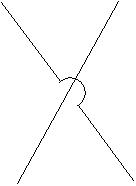
\includegraphics[scale=0.3]{OPE/1.jpg}\\
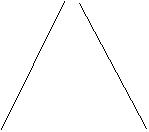
\includegraphics[scale=0.3]{OPE/2.jpg}\\
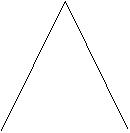
\includegraphics[scale=0.3]{OPE/3.jpg}\\
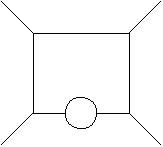
\includegraphics[scale=0.3]{OPE/4.jpg}\\
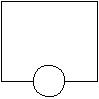
\includegraphics[scale=0.3]{OPE/5.jpg}\\
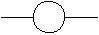
\includegraphics[scale=0.3]{OPE/6.jpg}\\
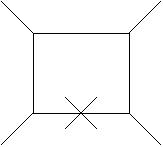
\includegraphics[scale=0.3]{OPE/7.jpg}\\
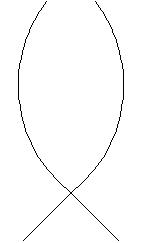
\includegraphics[scale=0.3]{OPE/openfish.jpg}\\
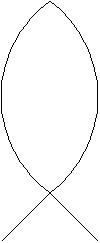
\includegraphics[scale=0.3]{OPE/closedfish.jpg}\\

\newpage

\bibliographystyle{ieeetr} 
\bibliography{opeBib.bib}

\end{document}
